\documentclass[tikz,border=10pt]{standalone}
\usetikzlibrary{intersections, calc}

\begin{document}
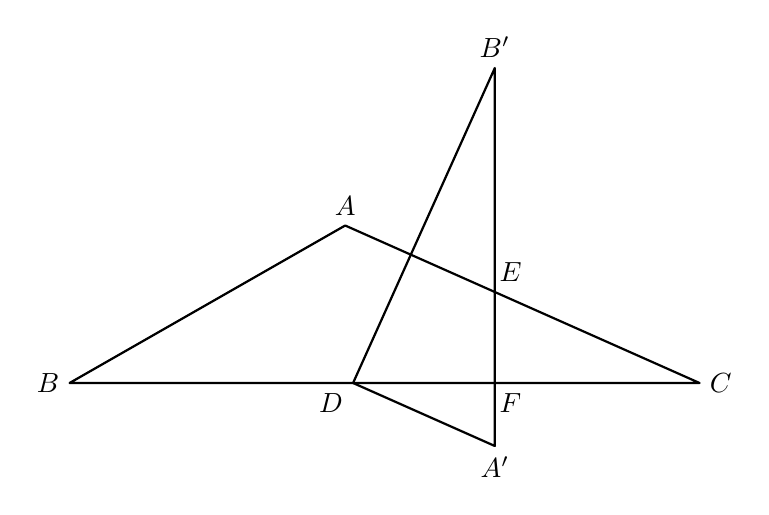
\begin{tikzpicture}[line join=round, line cap=round, >=stealth, thick]

    % --- 1. 定义初始顶点坐标 (根据视觉比例设定) ---
    \coordinate (B) at (0,0);
    \coordinate (C) at (8,0);
    \coordinate (A) at (3.5,2);
    \coordinate (D) at (3.6,0); % D点在BC上

    % --- 2. 绘制原始三角形 ABC ---
    \draw (A) -- (B) -- (C) -- cycle;

    % --- 3. 计算旋转/变换后的点 ---
    % 假设 A'B'D 是由 ABD 绕 D 点旋转并平移得到的，这里通过相对坐标精确还原图像结构
    \coordinate (Bprime) at (5.4,4);
    \coordinate (Aprime) at (5.4,-0.8);

    % --- 4. 绘制变换后的三角形 A'B'D ---
    \draw (D) -- (Bprime) -- (Aprime) -- cycle;

    % --- 5. 计算并标记交点 E 和 F ---
    % 定义路径用于求交点
    \path[name path=AC] (A) -- (C);
    \path[name path=BprimeAprime] (Bprime) -- (Aprime);
    \path[name path=BC] (B) -- (C);

    % 求 AC 与 A'B' 的交点 E
    \path [name intersections={of=AC and BprimeAprime, by=E}];
    % 求 BC 与 A'B' 的交点 F
    \path [name intersections={of=BC and BprimeAprime, by=F}];

    % --- 6. 标注文本标签 ---
    \node[above] at (A) {$A$};
    \node[left]  at (B) {$B$};
    \node[right] at (C) {$C$};
    \node[below left] at (D) {$D$};
    \node[above] at (Bprime) {$B'$};
    \node[below] at (Aprime) {$A'$};
    \node[above right, xshift=-2pt] at (E) {$E$};
    \node[below right, xshift=-2pt] at (F) {$F$};

\end{tikzpicture}
\end{document}